\documentclass[parskip=full*,fontsize=10pt,BCOR=0pt,DIV=15]{scrreprt}
%\usepackage[french]{babel}
\usepackage{scrlayer-scrpage}

\usepackage{ifthen}
\newboolean{freeconference}
\newboolean{studentvolunteer}
\newboolean{speaker}

% Conference configuration
\newcommand{\esugyear}{\the\year\xspace{}}
\newcommand{\esuglocation}{Montpellier, France\xspace{}}
\newcommand{\esugstartdate}{3rd Feb, \esugyear{}\xspace{}}
\newcommand{\esugenddate}{7th Feb, \esugyear{}\xspace{}}
% \newcommand{\campstartdate}{26th Aug, \esugyear\xspace{}}
%\newcommand{\esughosting}{ZweiDenker GmbH\xspace{}}
\newcommand{\esuglocalorganizer}{Dr. Oleksandr Zaitsev}
%\usepackage[french]{babel}
\usepackage[utf8]{inputenc}

% Personal configuration
\newcommand{\fullname}{Andrzej Prochyra}
\newcommand{\birthdate}{}
\newcommand{\birthplace}{}
\newcommand{\fulladdress}{}
\newcommand{\passport}{}
\setboolean{freeconference}{true}
\setboolean{studentvolunteer}{true}
\setboolean{speaker}{false}


\deftripstyle{esugpagestyle}{}{}{}{
  \begin{tabular}{l}
    ESUG \\ \url{http://www.esug.org}
  \end{tabular}
}{}{
  \begin{tabular}{rr}
    Association Loi  1901 n$^{\circ}$W751167780  (not subjected to  V.A.T.)\\
    c/o Mr. St\'ephane Ducasse - 1 rue Cesar Franck - 59800 Lille - France
  \end{tabular}
} \pagestyle{esugpagestyle}
\addtokomafont{pagefoot}{\small}


\usepackage{lmodern}
\usepackage[T1]{fontenc}
\usepackage{xspace}
\usepackage{microtype}
\usepackage[pdftex]{color,graphicx}
\usepackage{multirow}
\usepackage[pdftex, colorlinks=true]{hyperref}
\begin{document}

\begin{center}
  
\includegraphics[width=.4\textwidth]{esug-logo}
\end{center}

\begin{flushright}
  Lille, France, \today
\end{flushright}

\fullname\\
\ifthenelse{\equal{\birthplace}{}}{}{Born:, \birthplace\\}
%\fulladdress\ifthenelse{\equal{\fulladdress}{}}{}{Current Address:, \fulladdress}\\
\ifthenelse{\equal{\fulladdress}{}}{}{Address:, \fulladdress}\\
\ifthenelse{\equal{\passport}{}}{}{No Passport : \passport}\\

\textbf{\underline{Subject:}  Attestation of Presence at the isLoop 2025 Winter School}

Dear \fullname{},

I attest that you participated to the 3rd International School on Live Object-Oriented Programming (isLoop) that was held in Montpellier, France, from 3rd till 7th of February 2025 with a total duration of 40 academic hours (13 hours of lectures and 27 hours of guided practice). The school was locally organized by Dr. Oleksandr Zaitsev and hosted by UMR SENS (\url{https://umr-sens.fr/}).

Please visit the isLoop web site at \url{https://isloop.pharo.org/2025-montpellier/} to find more information about the event.

Sincerely,


\begin{tabular}{ll}
  St\'ephane Ducasse & \\
  stephane.ducasse@inria.fr&\\
  \multirow{7}{.5\textwidth}{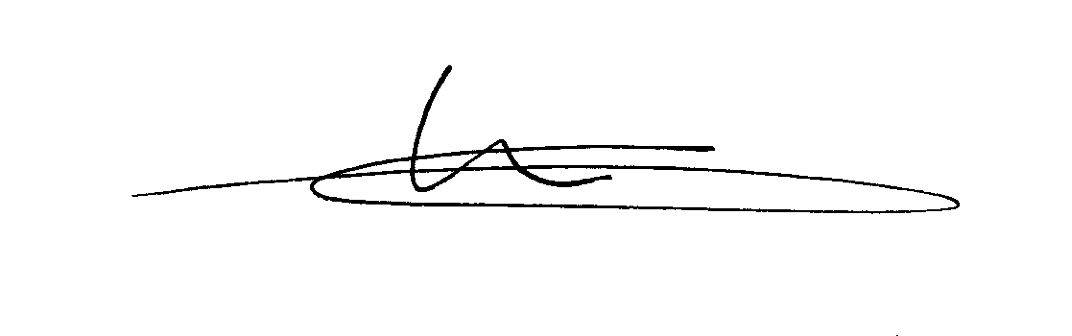
\includegraphics[width=.5\textwidth]{signature}} & Pr\'esident du groupe europ\'een d'utilisateurs de Smalltalk \\
& President of  the European Smalltalk User Group\\
&  ESUG \\
&  Inria Lille Nord Europe, 40, avenue Halley,\\
&  Parc Scientifique de la Haute Borne,\\
&   Bât.A, Park Plaza\\
&  Villeneuve d'Ascq  59650\\
&  France
\end{tabular}

\end{document}

%%% Local Variables:
%%% mode: latex
%%% TeX-master: t
%%% TeX-PDF-mode: t
%%% coding: utf-8
%%% ispell-local-dictionary: "english"
%%% End:
